
\documentclass[11pt,notitlepage]{article}

\usepackage{amsfonts, amsmath, amsthm, amssymb} % For math fonts
\usepackage{booktabs} % Top and bottom rules for table
\usepackage{wrapfig} % Allows in-line images
\usepackage[labelfont=bf]{caption} % Make figure numbering in captions bold
\usepackage{graphicx} % Required for including images
\usepackage[top=0.7in,bottom=1in,left=1in,right=1in]{geometry}
\pagestyle{empty} % Remove page numbering
\usepackage{float}
\usepackage{siunitx}
\newcommand{\tss}{\textsuperscript}
\newcommand{\tsbs}{\textsubscript}
\hyphenation{ionto-pho-re-tic iso-tro-pic fortran} % Specifies custom hyphenation points for words or words that shouldn't be hyphenated at all

%\sisetup{input-symbols ={()}, %do not treat ``(`` in tables differentl
%         group-digits = false}
\sisetup{
  per-mode = symbol,
  output-decimal-marker = {.},
  range-units = brackets,
  }

\renewcommand{\thesection}{\Roman{section}}

\begin{document}

\vspace*{0.5cm}

\noindent{\fontsize{16}{19.2}\selectfont \textbf{Contamination Spill
10/25/16} \\ Animal Industries Annex Room 20}

%------------------------------------------------------------
%	Incident
%------------------------------------------------------------
 
\section{Incident}
Around 11:00 am on Tuesday, October 25th, two small vials,
of the form shown in Figure \ref{fig:example2},
were loaded into a glovebox antechamber inside a glass beaker.
These two samples contained 469 $\pm$ 9.38 $\mu$l of 4 M HNO\tsbs{3}
and 430 $\pm$ 8.6 $\mu$l mixture of TBP (30 vol.\%) and kerosene.
The two vials were part of a Plutonium Uranium Redox EXtraction (PUREX)
experiment, with dissolved irradiated uranium fuel RSO 0079436.
The estimated gamma activities of the two vials is shown in
Table \ref{fig:activities}.

\begin{figure}[H] % Example of including images
\begin{center}
  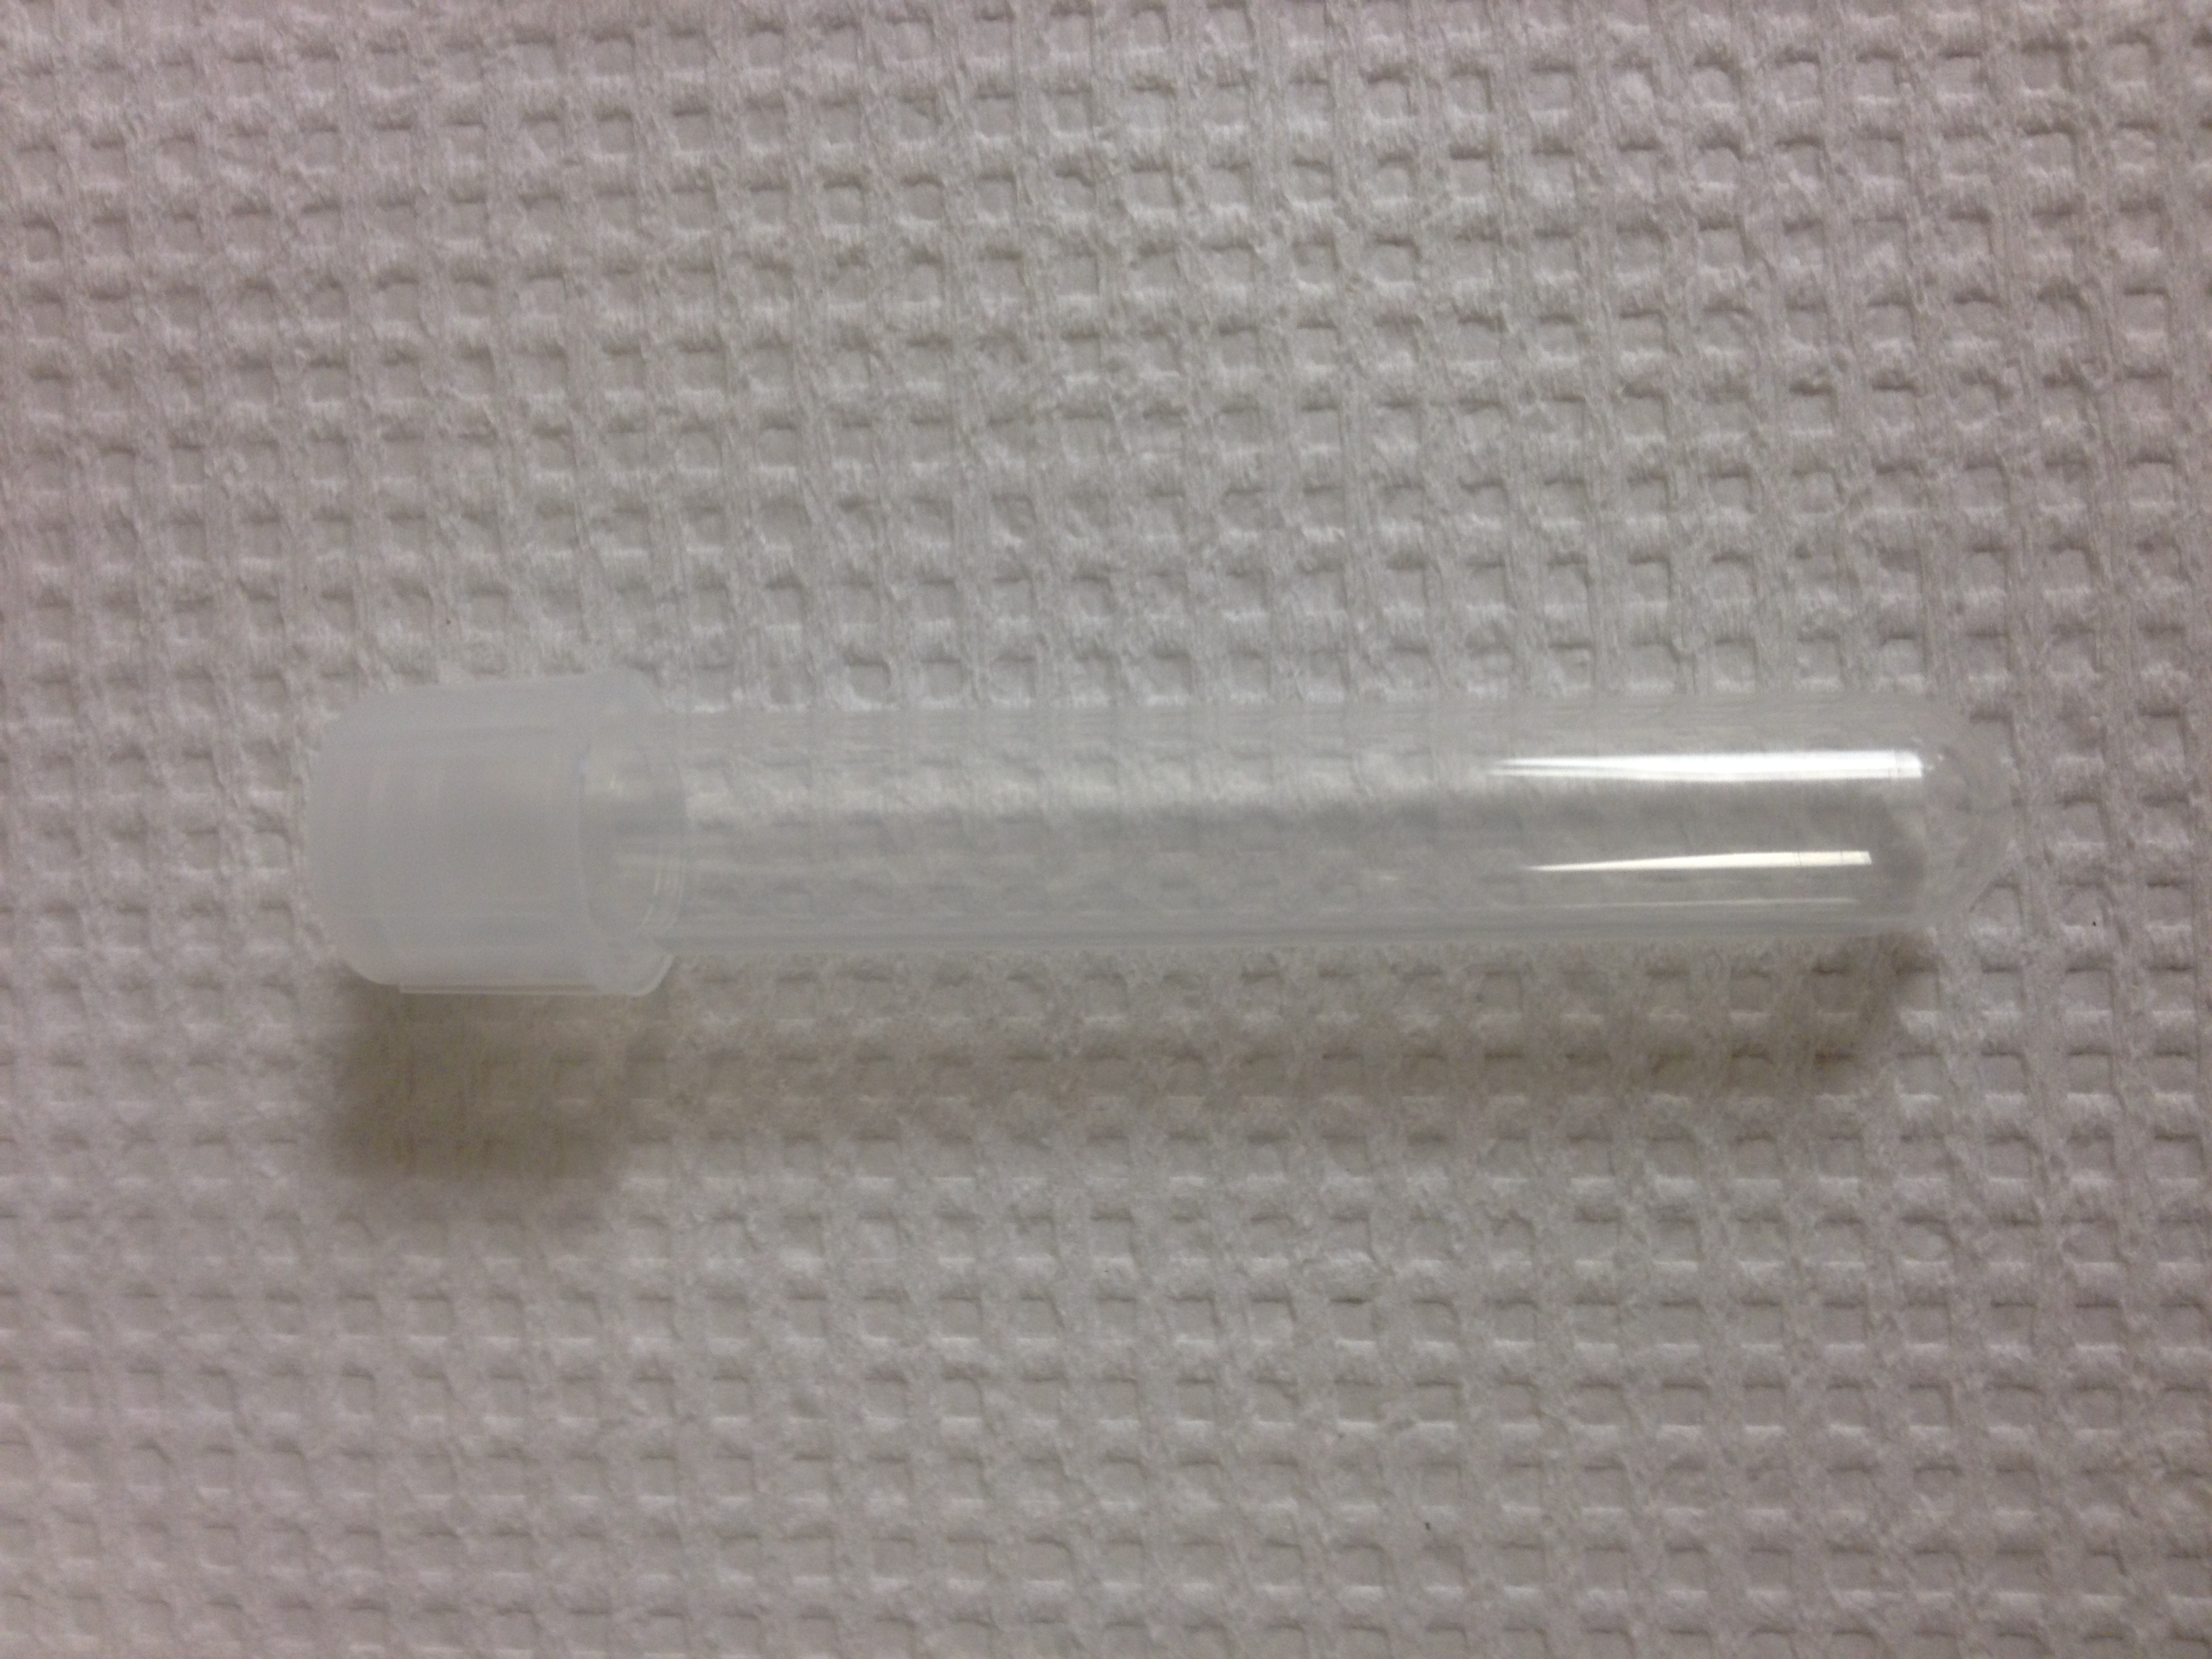
\includegraphics[width=0.75\linewidth]
                  {Figures/image1}
\end{center}
\caption{Image of vial type that leaked}
\label{fig:example2}
\end{figure}

\begin{table}[H]
  \begin{center}
    \caption{Activities in the two vials}
    
  \begin{tabular}{|c S[table-format=1.3] S[table-format=1.3] S[table-format=1.5] S[table-format=1.5] S[table-format=1.3] S[table-format=1.3]|}
    \hline
    Isotope
    & {HNO\tsbs{3} [$\mu$Ci]}
    & {$\pm$}
    & {TBP [$\mu$Ci]}
    & {$\pm$}
    & {Estimated Total [$\mu$Ci]}
    &  {$\pm$}
    \\
    \hline\hline
    \tss{144}Ce & 5.70 & 0.06 & 0.118 & 0.003 & 5.82 & 0.06\\
    \hline
    \tss{154}Eu & 0.054 & 0.002 & 0.0033 & 0.0002 & 0.057 & 0.002\\
    \hline
    \tss{125}Sb & 0.24 & 0.01 & 0.0007 & 0.0006 & 0.24 & 0.01\\
    \hline
    \tss{106}Rh & 6.3 & 0.3 & 0.240 & 0.005 & 6.5 & 0.4\\
    \hline
    \tss{134}Cs & 0.359 & 0.01 & 0.00018 & 0.00006 & 0.36 & 0.01\\
    \hline
    \tss{137}Cs & 4.58 & 0.1 & 0.0162 & 0.0001 & 4.6 & 0.1\\
    \hline
  \end{tabular}
  \label{fig:activities}
\end{center}
\end{table}

The pump was turned on and air was pumped out
of the antechamber
until the pressure reached approximately -100 kPa. At this
point a pop was heard, and positive pressure was reinstated
for the antechamber. Upon opening the antechamber, both
vials were observed to have popped out of the glass beaker and spilled on
absorbent paper, which was covering the
tray inside the antechamber. An image of the antechamber with
tray is shown in Figure \ref{fig:fig2}.

\begin{figure}[H] % Example of including images
\begin{center}
  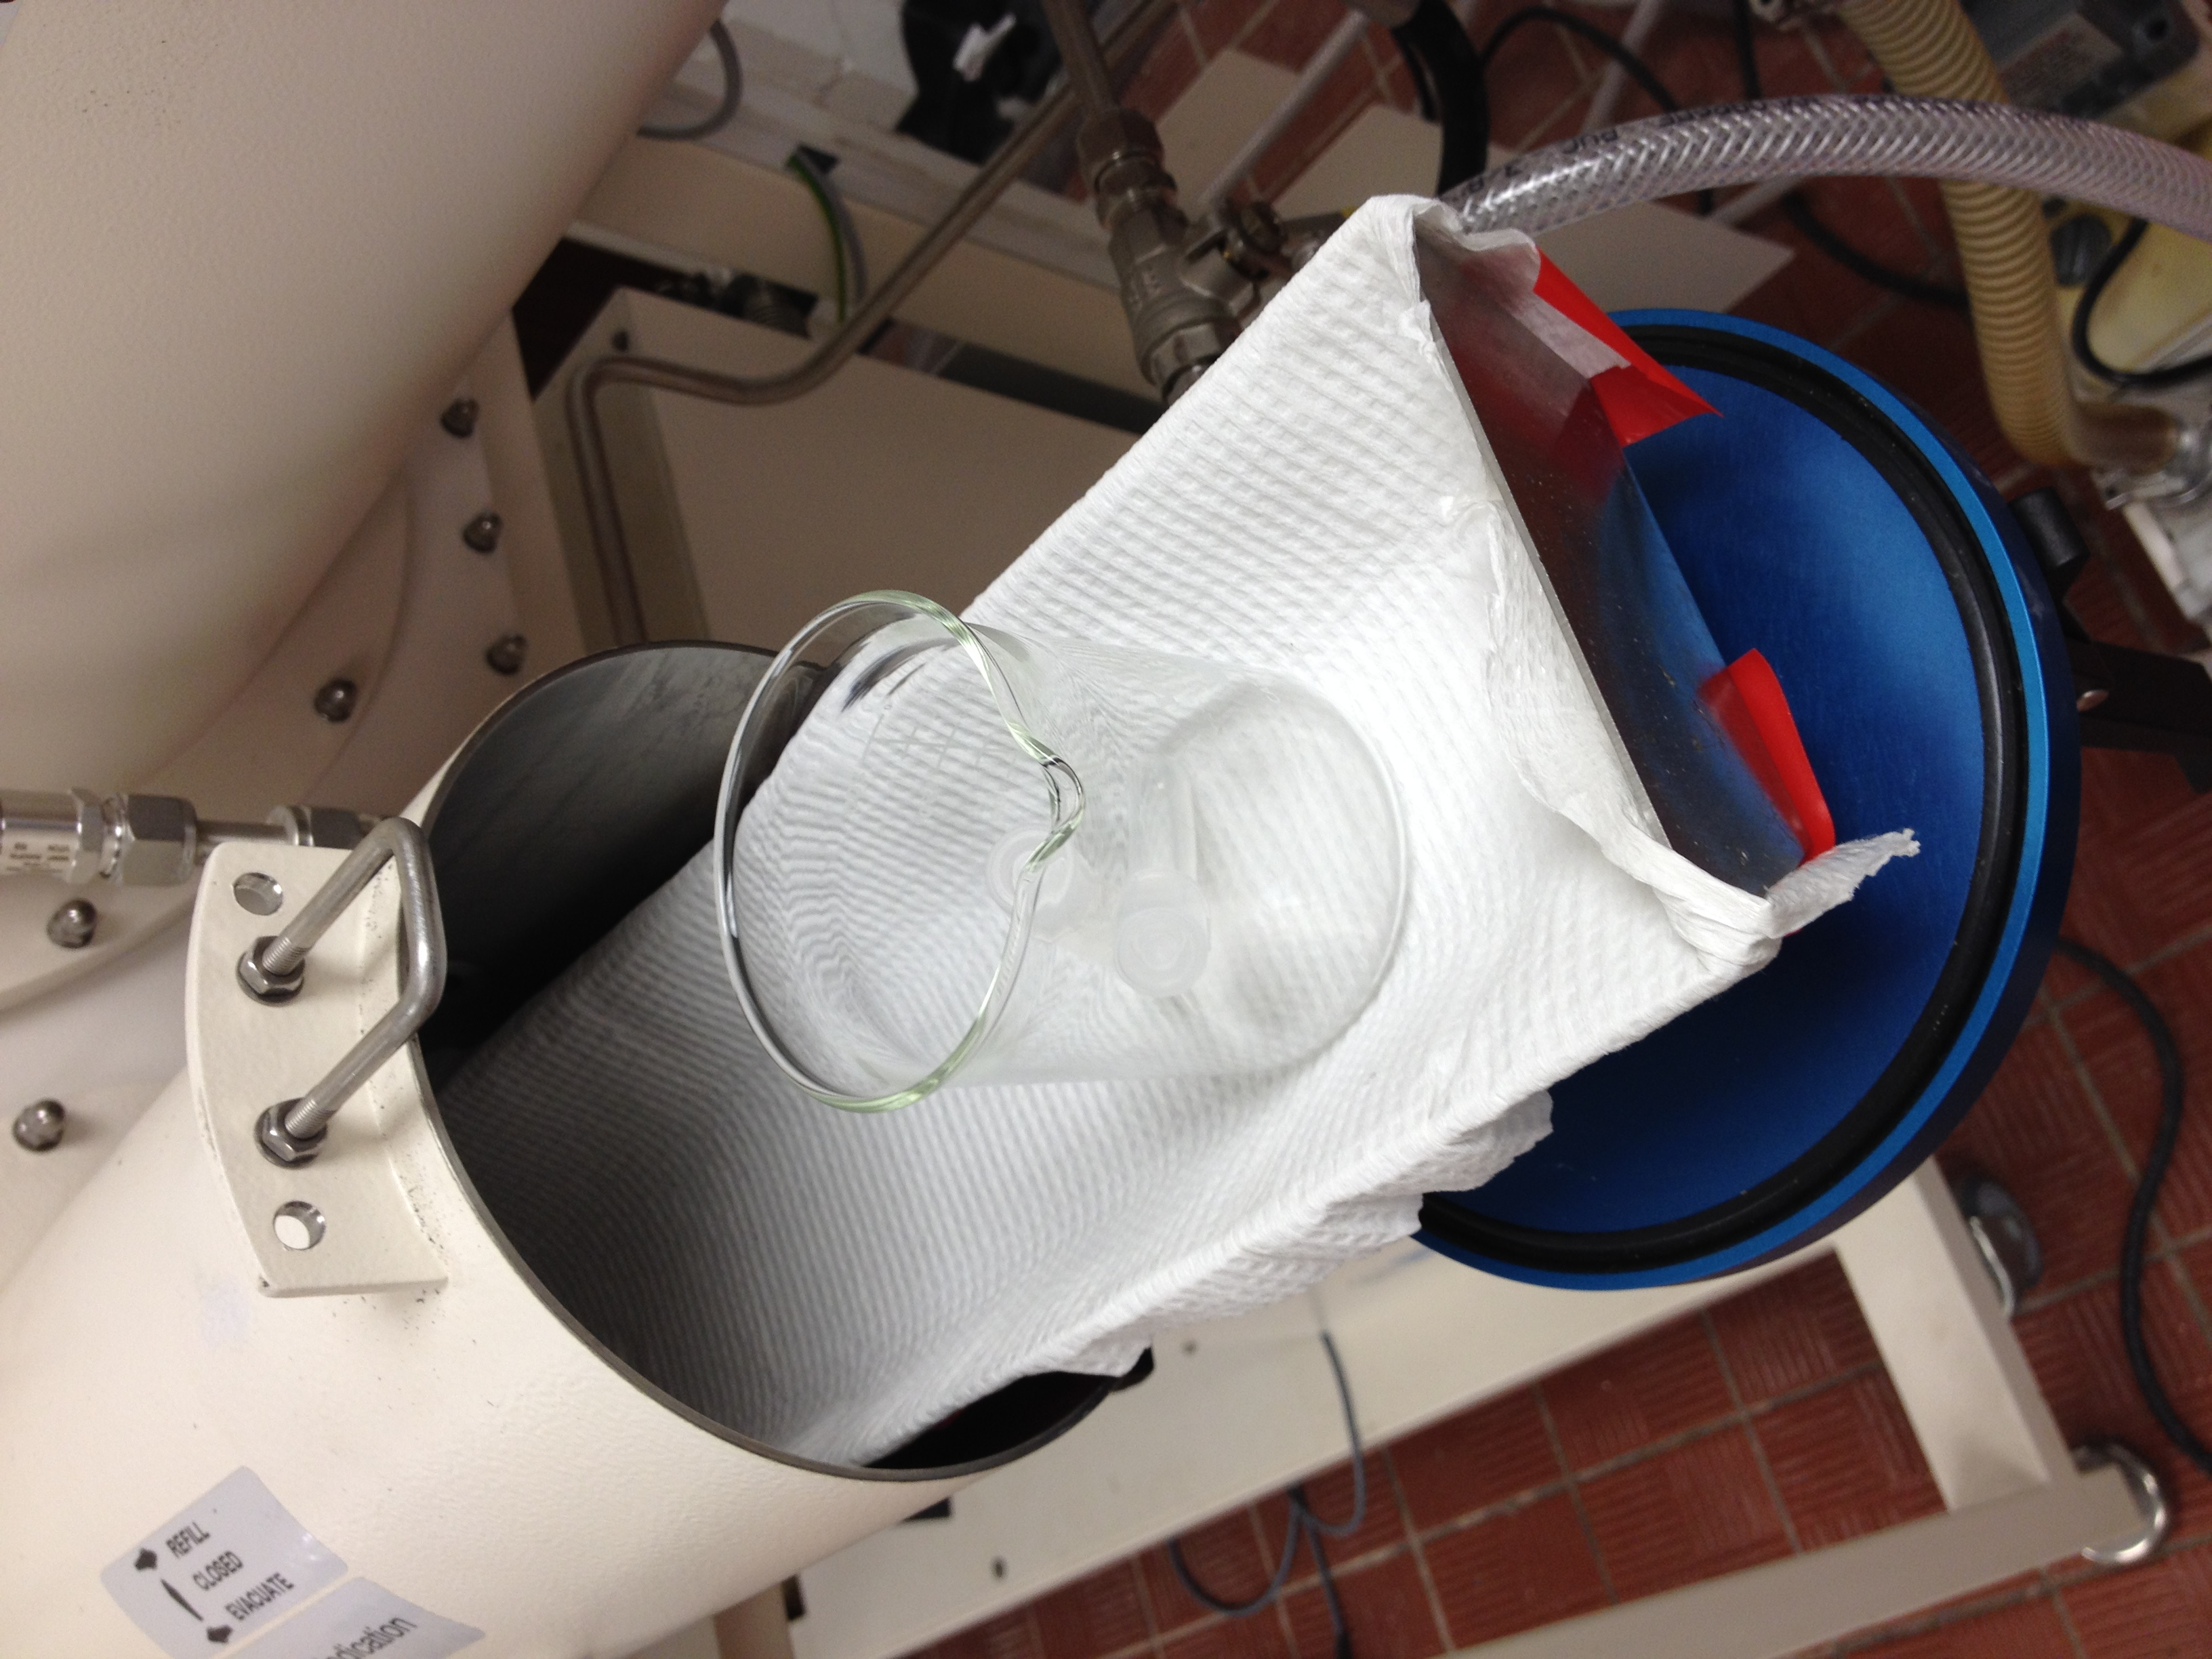
\includegraphics[angle=270,width=0.75\linewidth]
                  {Figures/image2}
\end{center}
\caption{Antechamber tray with diaper paper covering}
\label{fig:fig2}
\end{figure}

%------------------------------------------------------------
%	Initial Decontamination
%------------------------------------------------------------

\section{Decontamination}

Kevin Glennon performed the following tasks for the
initial decontamination:
\begin{itemize}
\item{Absorbent paper was layed down nearby and the two vials,
  with the glass beaker, were temporarily placed there
(until decontaminated)}
\item{The absorbent paper inside the antechamber was removed
  and thrown in the radioactive waste bin, and the tray was
  cleaned with radiacwash towelettes.}
\item{During this time, Paul was being scolded}
\end{itemize}
Both Paul and Kevin took swipes of several areas while
decontamination ensued. Swipes of the outlet to the antechamber
were clean \textit{before} decontamination and concerns
about radioactive material leaving the chamber to the pump
were low.
Keven left the lab and Paul
continued to decontaminate the antechamber and took
swipes of the area.
After decontamination the majority of the cylinder
of the antechamber was at background levels except the back
portion of the cylinder nearest the glovebox, which
were about 3 times background. Cleaning activities concluded
around 5:00 pm.

%------------------------------------------------------------
%	EHS Involvement
%------------------------------------------------------------

\section{EHS Involvement}

The following morning EHS was contacted and their assistance
was requested to clear the antechamber and pump for use.
Around 3:30 pm, Daniel Menchaca and Luis Rodriguez
arrived at the laboratory. After asking about exactly
what happened, they proceeded to swipe the area
around the glovebox and antechamber, including
the pump used for the antechamber. An alpha detector
was used to check for loose contamination and we were
asked to not work in the lab until the results for the swipes came in.
\\~\\
The following day (Friday), Luis informed me that the swipes were clean
and that work in the lab could continue, but not in the
glovebox until the antechamber was cleared. I asked if
I could continue to decontaminate the antechamber and he said that
was acceptable. 
\\~\\
On Monday, both Daniel and Luis arrived around 10:00 am to take
swipes of the antechamber. 
\\~\\
%------------------------------------------------------------
%	Presumed location of radioactive waste
%------------------------------------------------------------
After decontamination of the antechamber and taking swipes
of the area, it is assumed that the majority of the contamination
made its way to the radioactive waste.

%------------------------------------------------------------
%	Lessons learned
%------------------------------------------------------------

\section{Lessons learned}

This contamination spill is mostly due to procedural oversight
of Paul Mendoza. The experiments started this semester utilized
a different vial type than in previous experiments, and the
large vacuum created in the antechamber caused the new vials
to spill. Procedures for transferring samples into the glovebox
now entail that all samples need to be contained within a
vial type that has a screw top, and should be parafilm wrapped
as an extra precaution. 

\end{document}
